%!TeX spellcheck = en_UK
% Die erste (unkommentierte) Zeile im Dokument legt immer die
% Dokumentklasse fest
\documentclass{scrartcl} 

% Präambel:
% Einbinen von zusätzlichen Paketen. Falls für eine Datei keine Endung
% explizit angegeben wird, benutzt LaTeX '.tex'. Im Folgenden wird
% also die Datei 'edv_pakete.tex' eingebunden.
\input{edv_pakete}


% Verzeichnisse mit Abbildungen; kann gestrichen werden,
% falls Sie dies schon in edv_pakete.tex definiert haben:
%\graphicspath{{../report}}

\addbibresource{refs.bib} %Hinzufügen einer Literaturdatenbank aus dem angegebenen Verzeichnis

% Titel, Autor und Datum
\title{Computational Physics}
\subtitle{Exercise 2}
\date{\today}
\author{Christiane Groß, Nico Dichter}

% Jetzt startet das eigentliche Dokument
\begin{document}
	\maketitle
\section{The 2D-Ising-model}
We want to expand our solution of the Ising model in one dimension to two dimensions. For this the Hamiltoninan stays unchanged 
\begin{equation}
H(s)=-J\sum_{\langle i,j\rangle }s_is_j-h\sum_{\langle i,j\rangle }s_i
\label{eq:hamiltonianising}
\end{equation}

Here $J$ is the coupling between the nearest-neighbour-spins, $h$ is the value of the external magnetic field and the sum is over the entire lattice of size $\Lambda=N_x \cdot N_y$. In our simulations we always choose $N=N_x=N_y$.
We also know the theoretical expectation values for the  absolute value of the magnetization $|m|$ and the average energy per site $\epsilon$ when there is no external field present:
\begin{equation}
\epsilon=-J\coth(2J)\left( 1+\frac{2}{\pi}(2\tanh^2(2J)-1)K(4\sinh^2(2J)/\cosh^4(2J))\right) 
\end{equation}
\begin{equation}
|m|=\left( 1-\frac{1}{\sinh(2J)}\right)^{1/8} \text{ if } J<J_c,\quad 0 \text{ else}   
\end{equation}
 with $K(m)$ the incomplete elliptic integral of the first kind and the critical coupling $J_c=\frac{1}{2}\log(1+\sqrt{2})$. We simulate the elliptic integral with the gsl\_special-functions~\cite{gsldoc_sf}.
 
 Contrary to our simulation of the Ising model in one dimension, we do not do simple sampling here, but instead we do importance sampling. For this, we do a sweep of the entire lattice and perform an accept-reject step at each site: We propose a spin flip $s\rightarrow-s$ and accept it with probability $\min \left[1, \exp(-\Delta H/k_BT)\right]$, where $\Delta H$ is the change in energy due to the spin flip.  
%Hamiltonian, expected values for magnetization and epsilon

We furthermore know the theoretical value for the heat capacity:
\begin{equation}
C=\frac{4J^2}{\pi\tanh^2(2J)}\left( K(\kappa^2)-E(\kappa^2)-\left(1-\tanh^2(2J)\right)\left[\frac{\pi}{2} +\left(2\tanh^2(2J)-1\right)K(\kappa^2)\right] \right)
\end{equation}

where $E$ is the incomplete elliptical of the second kind and $\kappa=\frac{2\sinh(2J)}{\cosh^2(2J)}$.

\section{Deliberations}
Before starting the simulations, we have to think about several aspects in our code:
\subsection{Numerical cost of calculation}
\paragraph{Energy}
Determining th energy of a given spin configuration means determining the hamiltonian with eq.~\ref{eq:hamiltonianising}. For this we need to sum over all lattice points, so the numerical cost of this is proportional to the system size $\Lambda$.
% Have to iterate over all lattice points: effort proportional lambda.

\paragraph{Change in energy for one spin flip}
The naive approach to calculating the energy difference if one spin is flipped would be to calculate the hamiltoninan before and after the flip and subtract the results. This would scale with $\Lambda$. However, as was shown in the lectures, subtracting the hamiltonians leaves only the interactions with the nearest neighbours, because these are the only couplings we consider. There are four nearest neighbours in two dimensions, no matter how large the lattice is. so, the numerical cost of this calculation is constant, regardless of $\Lambda$.
%naive: calculate two Hamiltonians, subtract: scales with lambda. 
%Possible: only use nearest neighbours, as shown in lecture for 1D: effort only depends ion dimension, not lattice size.

\subsection{Meaning of $J_c$} 
We expect a phase transition to occur at $J=J_c$ and $h=0$: for smaller $J$, the magnetization will be zero and the spins will be randomly disributed. For $J>J_c$, most of the spins will be pointing in one direction and the magnetization will be much closer to one than to zero and measurable. The drop in magnetization is quite steep in theory, however, due to our finite lattice sizes, it is to be expected that this effect will be smeared out and we will see a continuous curve~\cite{YangMagnetization}\cite{binderheermann}.
%critical J: phase transition from randomly ordered to ordered.

\subsection{Determining errors}

Because we are doing importance sampling, we do not need to consider the partition function and can calculate expectation values as simple arithmetic means. This gives us:
\begin{equation}
\langle x\rangle=\frac{1}{L}\sum_{i=0}^{L} x_i
\end{equation}
\begin{equation}
\sigma^2(x)=\langle (\langle x\rangle-x)^2\rangle=\langle x^2\rangle-\langle x\rangle^2=\frac{1}{L}\sum_{i=0}^{L} x_i^2-\left( \frac{1}{L}\sum_{i=0}^{L} x_i\right) ^2
\label{eq:error}
\end{equation}

x is the observable we want to measure, so $m$ or $\epsilon$. We know these error estimates are a bit off due to correlation in the data, however for this sheet, no other methods of estimating errors were introduced in the lectures.

\subsection{Heat capacity}

From the sheet we know we can calculate $C$ as $C=\Lambda\cdot(\langle \epsilon^2\rangle-\langle \epsilon\rangle^2)$. So we need to measure the quantity $\langle \epsilon^2\rangle-\langle \epsilon\rangle^2$. However, looking at eq.~\ref{eq:error} we see that we have already calculated this as the error of $\epsilon$ and thus only need to multiply the square of the value we have already used with the system size $\Lambda$.

\section{Simulation}

Our code can be found in the github-repository \url{https://github.com/christianegross/CompPhys\_2021}. The simulation of the Ising model is in Exercise2/src/main/main.c, the calculations for the expected heat capacity and average energy are in Exercise2/report/epsilonexpected.c and the gnuplotscript for the plots is in Exercise2/report/plot.gp.

In the implementation of the simulation gsl\_matrix objects are used to save the state of the largest lattice and views on these are used to create smaller lattices (see \cite{gsldoc_mat}). For each parameter set (N,h,J) a large amount of thermalization sweeps are made and afterwards several measurements of the wanted physical variable take place with single sweeps in between. A Sweep in this case means scanning through the complete lattice and performing a Metropolis-Hastings step at each site. The thermalization steps are needed to make sure the measurements take place on configurations which resemble the given parameter set according to the boltzmann distribution. To improve the run time the function energy\_change was implemented. It calculates $\Delta S$ by only using the parts of the Hamiltonian which change when $s_{i,j}$ changes to $-s_{i,j}$, these parts consist of the energy of $s_{i,j}$ in the external magnetic field and the coupling energy with the 4 neighbours.
So in total $\Delta S$ simplifies to:
\begin{equation}
	\Delta S=2 s_{i,j}\left(\dfrac{h}{T}+\dfrac{J}{T}(s_{i+1,j}+s_{i-1,j}+s_{i,j+1}+s_{i,j-1})\right)
\end{equation}


\section{Results}

For all our results, we did the measurements with 1000 thermalisation steps and 2000 measurement steps per data point.

\subsection{$\langle m\rangle$ for fixed $J$ and varying $h$}
In fig.~\ref{fig:magfixJ}, our results are plotted for varying $h$ and $J=0.3$ and $J=0.8$. For $J=0.3<J_c$ we see a behaviour that is very similar to that of the ising model in one dimension: For $h=-1$, the magnetization is -1. It grows with $h$ and rises steeply in the region around $h=0$ and then grows slower, coming to $m=1$ at $h=1$. the rise is minimally less steep for $N=4$, all the measurements of the other $N$ lie on top of each other. The errors are bigger for smaller $N$ and biggest around $h=1$.
 
For $J=0.8>J_c$, the behaviour is quite different: From $h=-1$ to $h=-0.3$, the magnetization is minus one. Above that, the magnetization jumps to one, no value in between is seen. This underlines the phase transition that occurs at $J=J_c$: Below that critical value, the external magnetic field determines the strength of the magnetization as well as the direction of the spins. Above the critical coupling, the absolute value of the magnetization is fixed and can't be changed by external influences, the external fiel can only flip all spins at once.

	\begin{figure}[htbp]
		% GNUPLOT: LaTeX picture with Postscript
\begingroup
  \makeatletter
  \providecommand\color[2][]{%
    \GenericError{(gnuplot) \space\space\space\@spaces}{%
      Package color not loaded in conjunction with
      terminal option `colourtext'%
    }{See the gnuplot documentation for explanation.%
    }{Either use 'blacktext' in gnuplot or load the package
      color.sty in LaTeX.}%
    \renewcommand\color[2][]{}%
  }%
  \providecommand\includegraphics[2][]{%
    \GenericError{(gnuplot) \space\space\space\@spaces}{%
      Package graphicx or graphics not loaded%
    }{See the gnuplot documentation for explanation.%
    }{The gnuplot epslatex terminal needs graphicx.sty or graphics.sty.}%
    \renewcommand\includegraphics[2][]{}%
  }%
  \providecommand\rotatebox[2]{#2}%
  \@ifundefined{ifGPcolor}{%
    \newif\ifGPcolor
    \GPcolortrue
  }{}%
  \@ifundefined{ifGPblacktext}{%
    \newif\ifGPblacktext
    \GPblacktextfalse
  }{}%
  % define a \g@addto@macro without @ in the name:
  \let\gplgaddtomacro\g@addto@macro
  % define empty templates for all commands taking text:
  \gdef\gplbacktext{}%
  \gdef\gplfronttext{}%
  \makeatother
  \ifGPblacktext
    % no textcolor at all
    \def\colorrgb#1{}%
    \def\colorgray#1{}%
  \else
    % gray or color?
    \ifGPcolor
      \def\colorrgb#1{\color[rgb]{#1}}%
      \def\colorgray#1{\color[gray]{#1}}%
      \expandafter\def\csname LTw\endcsname{\color{white}}%
      \expandafter\def\csname LTb\endcsname{\color{black}}%
      \expandafter\def\csname LTa\endcsname{\color{black}}%
      \expandafter\def\csname LT0\endcsname{\color[rgb]{1,0,0}}%
      \expandafter\def\csname LT1\endcsname{\color[rgb]{0,1,0}}%
      \expandafter\def\csname LT2\endcsname{\color[rgb]{0,0,1}}%
      \expandafter\def\csname LT3\endcsname{\color[rgb]{1,0,1}}%
      \expandafter\def\csname LT4\endcsname{\color[rgb]{0,1,1}}%
      \expandafter\def\csname LT5\endcsname{\color[rgb]{1,1,0}}%
      \expandafter\def\csname LT6\endcsname{\color[rgb]{0,0,0}}%
      \expandafter\def\csname LT7\endcsname{\color[rgb]{1,0.3,0}}%
      \expandafter\def\csname LT8\endcsname{\color[rgb]{0.5,0.5,0.5}}%
    \else
      % gray
      \def\colorrgb#1{\color{black}}%
      \def\colorgray#1{\color[gray]{#1}}%
      \expandafter\def\csname LTw\endcsname{\color{white}}%
      \expandafter\def\csname LTb\endcsname{\color{black}}%
      \expandafter\def\csname LTa\endcsname{\color{black}}%
      \expandafter\def\csname LT0\endcsname{\color{black}}%
      \expandafter\def\csname LT1\endcsname{\color{black}}%
      \expandafter\def\csname LT2\endcsname{\color{black}}%
      \expandafter\def\csname LT3\endcsname{\color{black}}%
      \expandafter\def\csname LT4\endcsname{\color{black}}%
      \expandafter\def\csname LT5\endcsname{\color{black}}%
      \expandafter\def\csname LT6\endcsname{\color{black}}%
      \expandafter\def\csname LT7\endcsname{\color{black}}%
      \expandafter\def\csname LT8\endcsname{\color{black}}%
    \fi
  \fi
    \setlength{\unitlength}{0.0500bp}%
    \ifx\gptboxheight\undefined%
      \newlength{\gptboxheight}%
      \newlength{\gptboxwidth}%
      \newsavebox{\gptboxtext}%
    \fi%
    \setlength{\fboxrule}{0.5pt}%
    \setlength{\fboxsep}{1pt}%
\begin{picture}(8502.00,11904.00)%
    \gplgaddtomacro\gplbacktext{%
      \csname LTb\endcsname%
      \put(946,6656){\makebox(0,0)[r]{\strut{}$-1.5$}}%
      \put(946,7421){\makebox(0,0)[r]{\strut{}$-1$}}%
      \put(946,8185){\makebox(0,0)[r]{\strut{}$-0.5$}}%
      \put(946,8950){\makebox(0,0)[r]{\strut{}$0$}}%
      \put(946,9714){\makebox(0,0)[r]{\strut{}$0.5$}}%
      \put(946,10479){\makebox(0,0)[r]{\strut{}$1$}}%
      \put(946,11243){\makebox(0,0)[r]{\strut{}$1.5$}}%
      \put(1078,6436){\makebox(0,0){\strut{}$-1$}}%
      \put(2835,6436){\makebox(0,0){\strut{}$-0.5$}}%
      \put(4592,6436){\makebox(0,0){\strut{}$0$}}%
      \put(6348,6436){\makebox(0,0){\strut{}$0.5$}}%
      \put(8105,6436){\makebox(0,0){\strut{}$1$}}%
    }%
    \gplgaddtomacro\gplfronttext{%
      \csname LTb\endcsname%
      \put(176,8949){\rotatebox{-270}{\makebox(0,0){\strut{}$\langle m\rangle$}}}%
      \put(4591,6106){\makebox(0,0){\strut{}$h$}}%
      \put(4591,11573){\makebox(0,0){\strut{}$J=0.3$}}%
      \csname LTb\endcsname%
      \put(1738,11070){\makebox(0,0)[r]{\strut{}$N=$4}}%
      \csname LTb\endcsname%
      \put(1738,10850){\makebox(0,0)[r]{\strut{}$N=$8}}%
      \csname LTb\endcsname%
      \put(1738,10630){\makebox(0,0)[r]{\strut{}$N=$12}}%
      \csname LTb\endcsname%
      \put(1738,10410){\makebox(0,0)[r]{\strut{}$N=$16}}%
      \csname LTb\endcsname%
      \put(1738,10190){\makebox(0,0)[r]{\strut{}$N=$20}}%
    }%
    \gplgaddtomacro\gplbacktext{%
      \csname LTb\endcsname%
      \put(946,704){\makebox(0,0)[r]{\strut{}$-1.5$}}%
      \put(946,1469){\makebox(0,0)[r]{\strut{}$-1$}}%
      \put(946,2233){\makebox(0,0)[r]{\strut{}$-0.5$}}%
      \put(946,2998){\makebox(0,0)[r]{\strut{}$0$}}%
      \put(946,3763){\makebox(0,0)[r]{\strut{}$0.5$}}%
      \put(946,4527){\makebox(0,0)[r]{\strut{}$1$}}%
      \put(946,5292){\makebox(0,0)[r]{\strut{}$1.5$}}%
      \put(1078,484){\makebox(0,0){\strut{}$-1$}}%
      \put(2835,484){\makebox(0,0){\strut{}$-0.5$}}%
      \put(4592,484){\makebox(0,0){\strut{}$0$}}%
      \put(6348,484){\makebox(0,0){\strut{}$0.5$}}%
      \put(8105,484){\makebox(0,0){\strut{}$1$}}%
    }%
    \gplgaddtomacro\gplfronttext{%
      \csname LTb\endcsname%
      \put(176,2998){\rotatebox{-270}{\makebox(0,0){\strut{}$\langle m\rangle$}}}%
      \put(4591,154){\makebox(0,0){\strut{}$h$}}%
      \put(4591,5622){\makebox(0,0){\strut{}$J=0.8$}}%
      \csname LTb\endcsname%
      \put(1738,5119){\makebox(0,0)[r]{\strut{}$N=$4}}%
      \csname LTb\endcsname%
      \put(1738,4899){\makebox(0,0)[r]{\strut{}$N=$8}}%
      \csname LTb\endcsname%
      \put(1738,4679){\makebox(0,0)[r]{\strut{}$N=$12}}%
      \csname LTb\endcsname%
      \put(1738,4459){\makebox(0,0)[r]{\strut{}$N=$16}}%
      \csname LTb\endcsname%
      \put(1738,4239){\makebox(0,0)[r]{\strut{}$N=$20}}%
    }%
    \gplbacktext
    \put(0,0){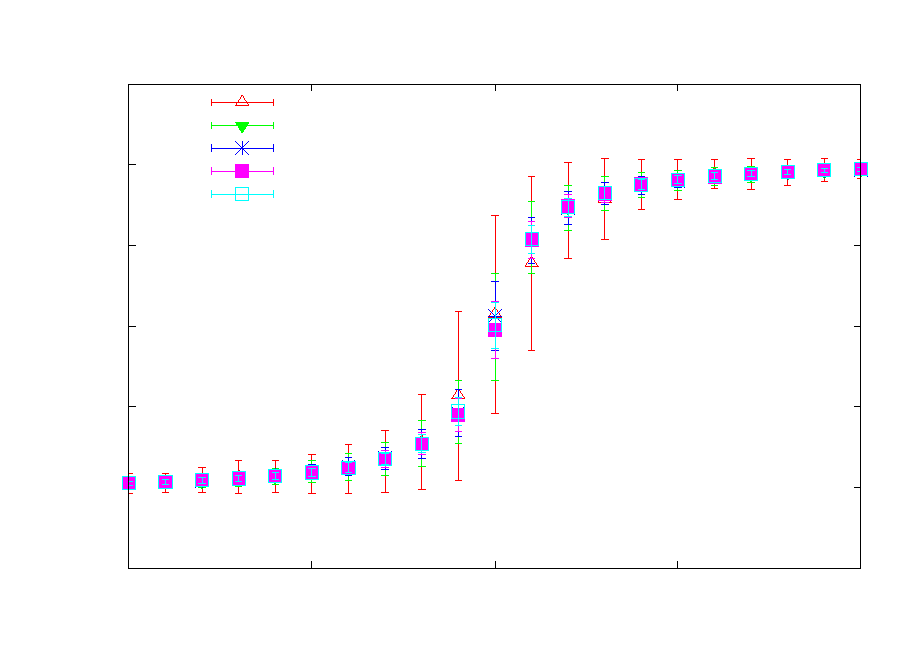
\includegraphics{magnetizationfixJ}}%
    \gplfronttext
  \end{picture}%
\endgroup

		\caption{Magnetization for two differerent values of fixed $J$}
		\label{fig:magfixJ}
	\end{figure}

\subsection{$\langle \epsilon\rangle$ for fixed $h=0$ and varying $J$}
We expect the average energy per site to fall monotonously, with a little curve at small J that then becomes a straight line. Up to about $J=0.45$, the values for $N=4$ are a bit below the expectation, the measurements for the other $N$ are at or above the expectation. The difference between the different $N$ is pretty small. From $J\approx0.45$, the measurements for all $N$ are below the expectations, but come closer with growing $J$. At $J=2$, the measurements lie on top of the expectation. 
	\begin{figure}[htbp]
		% GNUPLOT: LaTeX picture with Postscript
\begingroup
  \makeatletter
  \providecommand\color[2][]{%
    \GenericError{(gnuplot) \space\space\space\@spaces}{%
      Package color not loaded in conjunction with
      terminal option `colourtext'%
    }{See the gnuplot documentation for explanation.%
    }{Either use 'blacktext' in gnuplot or load the package
      color.sty in LaTeX.}%
    \renewcommand\color[2][]{}%
  }%
  \providecommand\includegraphics[2][]{%
    \GenericError{(gnuplot) \space\space\space\@spaces}{%
      Package graphicx or graphics not loaded%
    }{See the gnuplot documentation for explanation.%
    }{The gnuplot epslatex terminal needs graphicx.sty or graphics.sty.}%
    \renewcommand\includegraphics[2][]{}%
  }%
  \providecommand\rotatebox[2]{#2}%
  \@ifundefined{ifGPcolor}{%
    \newif\ifGPcolor
    \GPcolortrue
  }{}%
  \@ifundefined{ifGPblacktext}{%
    \newif\ifGPblacktext
    \GPblacktextfalse
  }{}%
  % define a \g@addto@macro without @ in the name:
  \let\gplgaddtomacro\g@addto@macro
  % define empty templates for all commands taking text:
  \gdef\gplbacktext{}%
  \gdef\gplfronttext{}%
  \makeatother
  \ifGPblacktext
    % no textcolor at all
    \def\colorrgb#1{}%
    \def\colorgray#1{}%
  \else
    % gray or color?
    \ifGPcolor
      \def\colorrgb#1{\color[rgb]{#1}}%
      \def\colorgray#1{\color[gray]{#1}}%
      \expandafter\def\csname LTw\endcsname{\color{white}}%
      \expandafter\def\csname LTb\endcsname{\color{black}}%
      \expandafter\def\csname LTa\endcsname{\color{black}}%
      \expandafter\def\csname LT0\endcsname{\color[rgb]{1,0,0}}%
      \expandafter\def\csname LT1\endcsname{\color[rgb]{0,1,0}}%
      \expandafter\def\csname LT2\endcsname{\color[rgb]{0,0,1}}%
      \expandafter\def\csname LT3\endcsname{\color[rgb]{1,0,1}}%
      \expandafter\def\csname LT4\endcsname{\color[rgb]{0,1,1}}%
      \expandafter\def\csname LT5\endcsname{\color[rgb]{1,1,0}}%
      \expandafter\def\csname LT6\endcsname{\color[rgb]{0,0,0}}%
      \expandafter\def\csname LT7\endcsname{\color[rgb]{1,0.3,0}}%
      \expandafter\def\csname LT8\endcsname{\color[rgb]{0.5,0.5,0.5}}%
    \else
      % gray
      \def\colorrgb#1{\color{black}}%
      \def\colorgray#1{\color[gray]{#1}}%
      \expandafter\def\csname LTw\endcsname{\color{white}}%
      \expandafter\def\csname LTb\endcsname{\color{black}}%
      \expandafter\def\csname LTa\endcsname{\color{black}}%
      \expandafter\def\csname LT0\endcsname{\color{black}}%
      \expandafter\def\csname LT1\endcsname{\color{black}}%
      \expandafter\def\csname LT2\endcsname{\color{black}}%
      \expandafter\def\csname LT3\endcsname{\color{black}}%
      \expandafter\def\csname LT4\endcsname{\color{black}}%
      \expandafter\def\csname LT5\endcsname{\color{black}}%
      \expandafter\def\csname LT6\endcsname{\color{black}}%
      \expandafter\def\csname LT7\endcsname{\color{black}}%
      \expandafter\def\csname LT8\endcsname{\color{black}}%
    \fi
  \fi
    \setlength{\unitlength}{0.0500bp}%
    \ifx\gptboxheight\undefined%
      \newlength{\gptboxheight}%
      \newlength{\gptboxwidth}%
      \newsavebox{\gptboxtext}%
    \fi%
    \setlength{\fboxrule}{0.5pt}%
    \setlength{\fboxsep}{1pt}%
\begin{picture}(8502.00,6008.00)%
    \gplgaddtomacro\gplbacktext{%
      \csname LTb\endcsname%
      \put(946,704){\makebox(0,0)[r]{\strut{}$-4$}}%
      \put(946,1334){\makebox(0,0)[r]{\strut{}$-3.5$}}%
      \put(946,1964){\makebox(0,0)[r]{\strut{}$-3$}}%
      \put(946,2594){\makebox(0,0)[r]{\strut{}$-2.5$}}%
      \put(946,3224){\makebox(0,0)[r]{\strut{}$-2$}}%
      \put(946,3853){\makebox(0,0)[r]{\strut{}$-1.5$}}%
      \put(946,4483){\makebox(0,0)[r]{\strut{}$-1$}}%
      \put(946,5113){\makebox(0,0)[r]{\strut{}$-0.5$}}%
      \put(946,5743){\makebox(0,0)[r]{\strut{}$0$}}%
      \put(1680,484){\makebox(0,0){\strut{}$0.4$}}%
      \put(2483,484){\makebox(0,0){\strut{}$0.6$}}%
      \put(3286,484){\makebox(0,0){\strut{}$0.8$}}%
      \put(4090,484){\makebox(0,0){\strut{}$1$}}%
      \put(4893,484){\makebox(0,0){\strut{}$1.2$}}%
      \put(5696,484){\makebox(0,0){\strut{}$1.4$}}%
      \put(6499,484){\makebox(0,0){\strut{}$1.6$}}%
      \put(7302,484){\makebox(0,0){\strut{}$1.8$}}%
      \put(8105,484){\makebox(0,0){\strut{}$2$}}%
    }%
    \gplgaddtomacro\gplfronttext{%
      \csname LTb\endcsname%
      \put(176,3223){\rotatebox{-270}{\makebox(0,0){\strut{}$\langle\epsilon\rangle$}}}%
      \put(4591,154){\makebox(0,0){\strut{}$J$}}%
      \put(4591,5633){\makebox(0,0){\strut{}}}%
      \csname LTb\endcsname%
      \put(7118,5570){\makebox(0,0)[r]{\strut{}theory}}%
      \csname LTb\endcsname%
      \put(7118,5350){\makebox(0,0)[r]{\strut{}$N=$4}}%
      \csname LTb\endcsname%
      \put(7118,5130){\makebox(0,0)[r]{\strut{}$N=$8}}%
      \csname LTb\endcsname%
      \put(7118,4910){\makebox(0,0)[r]{\strut{}$N=$12}}%
      \csname LTb\endcsname%
      \put(7118,4690){\makebox(0,0)[r]{\strut{}$N=$16}}%
      \csname LTb\endcsname%
      \put(7118,4470){\makebox(0,0)[r]{\strut{}$N=$20}}%
    }%
    \gplbacktext
    \put(0,0){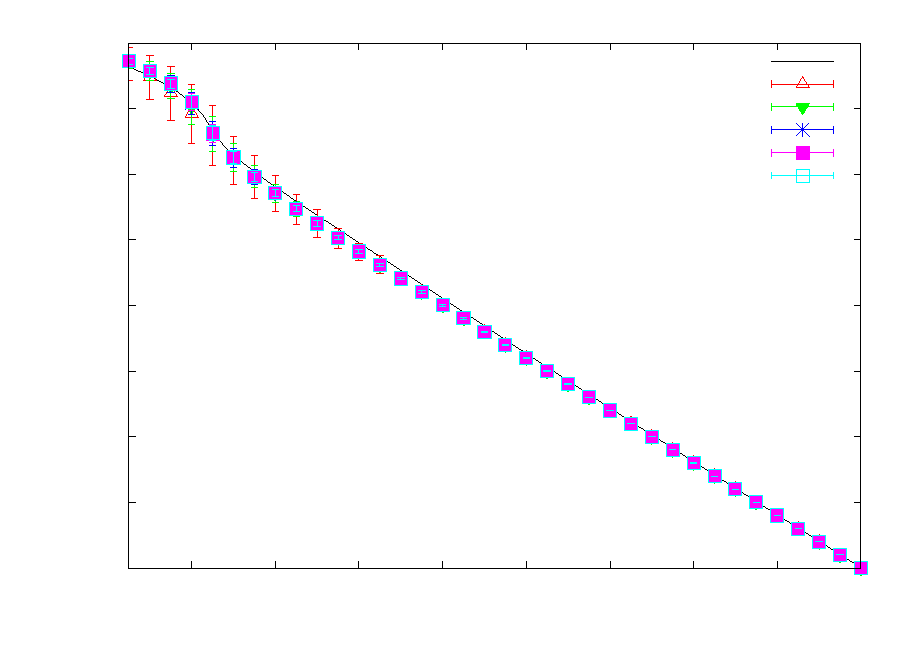
\includegraphics{avenergy}}%
    \gplfronttext
  \end{picture}%
\endgroup

		\caption{Average energy per site for $h=0$}
		\label{fig:energy}
	\end{figure}

\subsection{$\langle |m|\rangle$ for fixed $h$ and varying $J$}
plot, description, comparison literature

	\begin{figure}[htbp]
		\input{absmagnetization}
		\caption{Modulus of magnetization for $h=0$}
		\label{fig:absmag}
	\end{figure}
see sharp drop, phase transition
\paragraph{$\langle |m|\rangle$ vs. $\langle m\rangle$}
For $h=0$: everything cancels out, m=0 everywhere because simulation randomly flops between positive and negative behaviour, even at ordered phase due to finite length.
Use absolute value of m so it can't cancel out.

\paragraph{thermodynamical limit}

\subsection{heat capacity}

	\begin{figure}[htbp]
		\input{heatcapacity}
		\caption{Heat capacity for $h=0$}
		\label{fig:heat}
	\end{figure}

\newpage	
\listoffigures
\printbibliography
\end{document}